\section{Surrogate-based likelihoods}\label{sec:likelihoods}

Having obtained a stochastic surrogate model $y_D$, we wish to utilize it to evaluate the likelihood of the problem.

A first approach consists of considering the mean prediction of the surrogate model as a response surface and use that in the likelihood~\eqref{eq:likelihood} evaluations. 
For a mean prediction $m_D$, this corresponds to a parameter-to-observation relation 
\begin{equation}\label{eq:plug-in-par-to-obs}
    Y^m = m_D(p) + N
\end{equation}
and results in the likelihood
\begin{equation}\label{eq:plug-in-likelihood}
    L_{\text{plug-in}}(p) = \pi_N(y^m - m_D(p)).
\end{equation}
This is the so-called plug-in likelihood, which is a frequent choice in the literature~\cite{SinsbeckNowak2017}. 

However, this approach does not take into account the uncertainty of the surrogate model, which can lead to overconfident predictions and biased estimates of the parameters.
As we assume to be working with partial knowledge about the forward model $y$ only, our information about the relation between observation and parameters will also be limited. 
Relation~\eqref{eq:par-to-obs} may hold for the true forward map $y$, but as only a set $\{y_i\}_{i=1}^n$ of evaluations up to a certain accuracy is available, it is of little practical use. 
Thanks to the assumptions required by GPR and LR new relations can be obtained, incorporating the uncertainty about the forward model and resulting in surrogate-dependent likelihoods, $L_{D, \text{GP}}$ and $L_{D, \text{LR}}$ respectively. 

Having obtained a surrogate-based likelihood $L_D$, we can reformulate the posterior~\eqref{eq:Bayes} into 
\begin{equation} \label{eq:surr-posterior}
    \pi_{P\mid D, Y^m = y^m}(p) = \frac{L_D(p) \pi_P(p)}{\int_\Theta  L_D(p) \pi_P(p) \ dm_\Theta(p)},
\end{equation}
obtaining the Bayesian surrogate-informed posterior.

The remainder of this section first describes the surrogate-based likelihood for GPR, discussing the corresponding parameter-to-observation relation, and then the one for LR, deriving an implicit general formula and a closed-form expression for the uncorrelated-components noise case.

\subsection{GPR-based likelihood}\label{sec:GPlike}
By the assumptions of Section~\ref{sec:GPR}, when performing GPR one assumes the forward model to be a realization of a Gaussian process $Y$.
Incorporating this into the Relation~\eqref{eq:par-to-obs} leads to a different parameter-to-observation relation
\begin{equation}\label{eq:GPR-par-to-obs}
    Y^m = Y_p + N.
\end{equation}
Under normality and independence assumptions this results in a different likelihood, as stated in the following proposition.

\begin{prp}
    Let Relation~\eqref{eq:GPR-par-to-obs} hold with Gaussian noise $N \sim \mc N (0, \Sigma_N^2)$, let $y^m$ be a realization of $Y^m$ and let $y_{D, \text{GP}}$ be a GPR surrogate model describing the posterior distribution of $Y_p \sim \mc N( m_D(p), k_D(p,p) )$ given training data $D = \{ (p_i, \tau_i, y_i) \}_{i=1}^n$.

    Under the hypothesis that the GP prediction $Y_p$ is independent from the measurement noise $N$, Relation~\eqref{eq:GPR-par-to-obs} yields that $Y^m$ is normally distributed,
    \[
    Y^m \sim \mc N(m_D(p), \Sigma_N^2 + k_D(p,p)), 
    \]
    and consequently the marginal GPR likelihood of a parameter $p$ given measurements $y^m$ is given by
    \begin{equation}\label{eq:GPR-likelihood}
        L_{D, \text{GP}}(p) = (2\pi)^{-\frac{\text{dim} \mc Y}{2}} \text{det}\big ( \Sigma_N^2 + k_D(p, p) \big )^{-\frac{1}{2}} \exp \Big( -\frac{1}{2}\norm{y^m - m_D(p)}_{(\Sigma_N^2 + k_D(p,p))^{-1}}^2 \Big ).
    \end{equation}
\end{prp}
\begin{proof}
    The sum of independent multivariate normal variables $\eta_1, \ \eta_2$, with $\eta_i \sim \mc N(m_i, \Sigma^2_i)$, is again a normal variable of distribution $\mc N ( m_1 + m_2, \Sigma_1^2, \Sigma_2^2)$.
    Consequently from Relation~\eqref{eq:GPR-noise-corr} and the independence of $Y_p$ and $N$, we have that $Y^m$ is normally distributed with mean $m_D(p)$ and covariance $\Sigma_N^2 + k_D(p,p)$. \newline
    As $L_{D, \text{GP}}(p)$ is the density of $Y^m$ at $y_m$ as a function of $p$, one obtains Equation~\eqref{eq:GPR-likelihood} from the density of a multivariate normal distribution.
\end{proof}
\begin{rmk}
    The marginal GPR likelihood is the marginal distribution for $Y^m$ of the joint distribution of $Y^m$ and $Y(p)$:
    \begin{equation*}
        L_{D}(p) =  \mathbb E_{Y_p} \Big [ \pi_N (y^m - Y_p) \Big ],
    \end{equation*}
    justifying the name marginal likelihood.
\end{rmk}

As the prediction of GPR is stochastic, it is reasonable that likelihood of observing $y^m$ depends not only on the mean $m_D$, but also on the variance $k_D$. 
This is reflected in the surrogate-informed likelihood~\eqref{eq:GPR-likelihood}, which by having an higher variance is less prone to produce an overconfident posterior.
Adopting the marginal likelihood includes more information about the forward model, but results in a more complicated likelihood function when compared to the plug-in likelihood~\eqref{eq:plug-in-likelihood}; as the covariance of the marginal likelihood depends on $p$, the posterior~\ref{eq:surr-posterior} can present more local minima and non-convex behavior. \newline
Picture~\ref{fig:GP-likelihoods} compares the plug-in and the marginalized likelihoods for a simple one-dimensional case.
\begin{figure}[H] 

    \begin{center}
    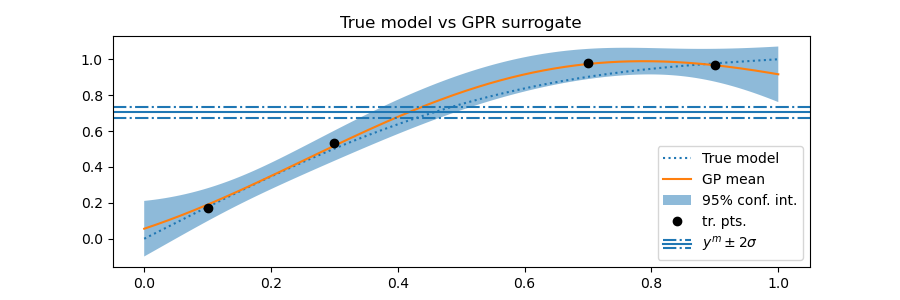
\includegraphics[width = 360pt]{results/pictures/d1/GP_model_comparison.png}
    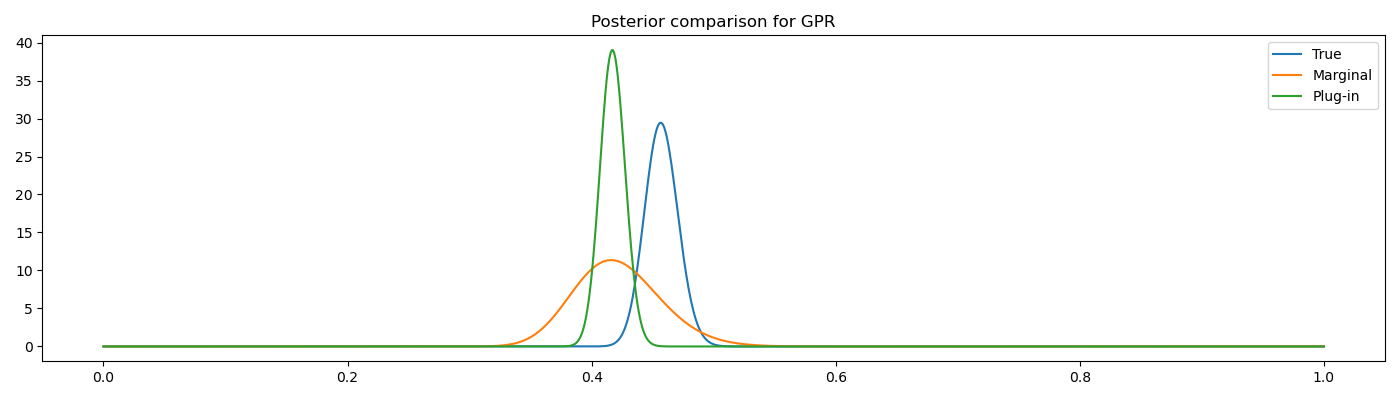
\includegraphics[width = 360pt]{results/pictures/d1/GP_posterior_comparison.png}
    \end{center}
    
    \caption{Impact of the plug-in likelihood~\eqref{eq:plug-in-likelihood} and GPR-based marginal likelihood~\eqref{eq:GPR-likelihood} on the posterior for an illustrative inverse problem problem with forward model $y(p) = p +\frac{1}{4} sin(\pi \cdot p)$ and Gaussian prior $\mc N(\frac{1}{2}, \frac{1}{3})$ on the parameter space $[0,1]$. The horizontal line in the first picture represents the measurement $y^m$ with the confidence interval of width $4 \cdot \sigma$, where $\sigma = 0.05$ is the measurement's standard deviation. The marginal likelihood~\eqref{eq:GPR-likelihood} is wider due to including the GP variance, and avoids an overconfident posteriors.} 
    \label{fig:GP-likelihoods}
\end{figure}  


\subsection{LR-based likelihood}\label{sec:LRlike}

Under the assumptions described in Section~\ref{sec:LR}, we can treat Relation~\eqref{eq:par-to-obs} similarly as done for GPR. 

Remind that, given training data $D =\{ (p_i, \tau_i, y_i) \}_{i=1}^n$, LR provides a predictive uniform distribution over some convex set $\mc PI_p \subseteq \mc Y $.
Marginalizing the likelihood over this predictive distribution leads to a marginal likelihood $L_{D, \text{LR}}(p)$ as given by the following proposition.

\begin{prp}\label{prp:LR-likelihood}
    Let $y_{D, \text{LR}}$ be a LR surrogate model as given in Definition~\ref{dfn:LR}, then if the prediction $Y_p \sim \mc U (\mc IP_p)$ is independent from the noise term $N$, the LR parameter-to-observation relation 
    \begin{equation*}
        Y^m = Y_p + N 
    \end{equation*}
    yields the marginal LR likelihood
    \begin{equation}\label{eq:LR-likelihood}
        L_{D, \text{LR}}(p) = \frac{1}{m_\mc Y (\mc PI_p)} \mathbb P \Big ( N \in \mc PI_p - y^m \Big ).
    \end{equation}
\end{prp}
\begin{proof}
    To obtain the density probability density $\pi_{Y^m}$ of $Y^m$ as in the statement, we recall the definition:
    \[ 
    \bb P\big(Y^m \in A\big) = \int_{A} \pi_{Y^m}(y) \ dy
    \] must hold for any measurable set $A \in \mc B \mc( Y)$. \newline
    For arbitrary $A \in \mc B(\mc Y)$, we write $\tilde A = \big \{ (y,n) \in \mc Y^2 \mid y + n \in A \big \}$ and obtain the following equalities: 
    \begin{flalign*}
        \bb P\big (Y^m \in A\big) &\stackrel{(1)}{=} \bb P\big(Y_p + N \in A\big) \stackrel{(2)}{=} \bb P \big( (Y_p, N) \in \tilde{A}\big) \stackrel{(3)}{=} \int_{\tilde{A}} \pi_{(Y_p, N)} (y, n) \, d(y,n) \stackrel{(4)}{=} && \\
        &\stackrel{(4)}{=} \int_{\mc Y} \pi_{Y_p} (y) \int_{A-y} \pi_{N}(n) \, dn \, dy \stackrel{(5)}{=} \int_{\mc Y} \pi_{Y_p} (y) \int_{A} \pi_{N}(\tilde n - y) \, d\tilde n \, dy \stackrel{(6)}{=} &&\\
        & \stackrel{(6)}{=} \int_{A} \int_{\mc Y} \pi_{Y_p} (y) \pi_{N}(\tilde n - y) \, dy \, d\tilde n \stackrel{(7)}{=}\int_{A} \bb E_{Y_p} \Big [ \pi_{N}(\tilde n - Y_p) \Big ] \, d\tilde n, &&
    \end{flalign*}
    where Equality~(1) used the parameter-to-observation relation, Equality~(2) used an equivalent reformulation of the set to be measured, Equality~(3) used the definition of the joint distribution of $Y_p$ and $N$, Equality~(4) used Fubini's Theorem and the independence of $Y_p$ and $N$, Equality~(5) used the change of variable $\tilde n = n + y$, Equality~(6) switched the order of integration by Fubini's Theorem, and Equality~(7) used the definition of expected value. \newline
    This chain of equalities deals \[
        \pi_{Y^m}(y) = \bb E_{Y_p} \Big [ \pi_{N}(y - Y_p) \Big ].
    \]
    To obtain the expression for $\pi_{Y^m}(y)$, we write
    \begin{flalign*}
        \pi_{Y^m} (y^m) &= \bb E_{Y_p} \Big [ \pi_{N}(y - Y_p) \Big ] \stackrel{(1)}{=} \int_{\mc Y } \frac{1_{\mc PI_p}(y)}{m_\mc Y (\mc PI_p)} \pi_{N}(y^m - y) \ dy \stackrel{(2)}{=} \frac{1}{m_\mc Y (\mc PI_p)} \int_{\mc P I_p  - y^m} \pi_{N}(e )  \ de \stackrel{(3)}{=} &&\\
        & \stackrel{(3)}{=} \frac{1}{m_\mc Y (\mc PI_p)} \mathbb P \Big ( N \in   \mc PI_p - y^m \Big  )&&,
    \end{flalign*}
    where Equality~(1) used the expression of the predictive distribution $\pi_{Y_p}$ given by Definition~\ref{dfn:LR}, Equality~(2) used the change of variable $e = y - y^m$ and the definition of indicator function, and Equality~(3) used the definition of the probability density function with $N$. \newline
    As the likelihood $L_{D, \text{LR}}(p)$ is the density of $Y^m$ at $y^m$ as a function of $p$, the statement follows.
\end{proof}

The efficiency in computing the likelihood~\eqref{eq:LR-likelihood} depends on the distribution of the measurement noise $N$ and the shape of $\mc P I_p  $.
For Gaussian measurement noise $N$ with independent components and $\mc PI_p$ being a rectangle, the likelihood can be computed as the product of differences of Gaussian cumulative distribution functions, as stated in the next proposition.

\begin{prp}
    In the hypothesis of Proposition~\ref{prp:LR-likelihood}, let  $N \sim \mc N (0, \Sigma^2_N)$ be Gaussian with $\Sigma_N = \text{diag} (\sigma_1, \ldots, \sigma_m)$, and let $\mc PI_p = \bigoplus_{j=1}^{\text{dim}\mc Y} \left[ LB^{(j)}(p), UB^{(j)}(p)\right] $.
    Then the LR likelihood~\eqref{eq:LR-likelihood} can be computed as 
    \[
        L_{D, \text{LR}}(p) = \prod_{j=1}^{\text{dim}\mc Y} \frac{\varphi \left( \frac{UB^{(j)}(p) - y^m}{\sigma_j} \right) - \varphi\left( \frac{LB^{(j)} - y^m}{\sigma_j} \right)}{UB^{(j)}(p) - LB^{(j)}(p)},
    \]
    where $\varphi$ is the standard normal cumulative distribution function.

\end{prp}
\begin{proof}
    By Proposition~\ref{prp:LR-likelihood} we can write 
    \[
        L_{D, \text{LR}}(p) = \frac{1}{m_\mc Y (\mc PI_p)} \mathbb P \Big ( N \in   \mc PI_p - y^m \Big ),
    \]
    then as $\mc PI_p$ is a rectangle and the components $N^{(1)}, \dots N^{(\text{dim} \mc Y)}$ of $N$ are independent, we can split the probability into the product of the probabilities of each component:
    \begin{flalign*}
        \mathbb P & \Big (  N \in   \mc PI_p - y^m  \Big ) = \mathbb P \Big ( N \in  \oplus_{j=1}^{\text{dim}\mc Y} \left[ LB^{(j)}(p) - y^m , UB^{(j)}(p) - y^m\right]  \Big ) = &&\\
        &= \prod_{j=1}^{\text{dim}\mc Y} \mathbb P \Big ( N^{(j)} \in  \left[ LB^{(j)}(p) - y^m , UB^{(j)}(p) - y^m\right]  \Big ) = \prod_{j=1}^{\text{dim}\mc Y} \varphi \left( \frac{UB^{(j)}(p) - y^m}{\sigma_j} \right) - \varphi\left( \frac{LB^{(j)} - y^m}{\sigma_j} \right), &&
    \end{flalign*}
    where the last equality follows from the definition of the cumulative distribution function $\varphi$.\newline
    Finally, we observe that the measure of the rectangle $\mc PI_p$ is given by \[
    m_{\mc Y}(\mc PI_p) = \prod_{j=1}^{\text{dim}\mc Y} \left( UB^{(j)}(p) - LB^{(j)}(p) \right),
    \] and then splitting the product deals the statement.
\end{proof}

\begin{rmk}
    Proposition~\ref{prp:LR-PI} states sufficient conditions for the predictive interval $\mc PI_p$ to be a multi-dimensional interval and provides the explicit formula to compute the bounds.
\end{rmk}

As for the GPR case, the marginal likelihood is more complicated than the plug-in likelihood, but it is more informative and less prone to bias. 
\begin{figure}[H] 

    \begin{center}
    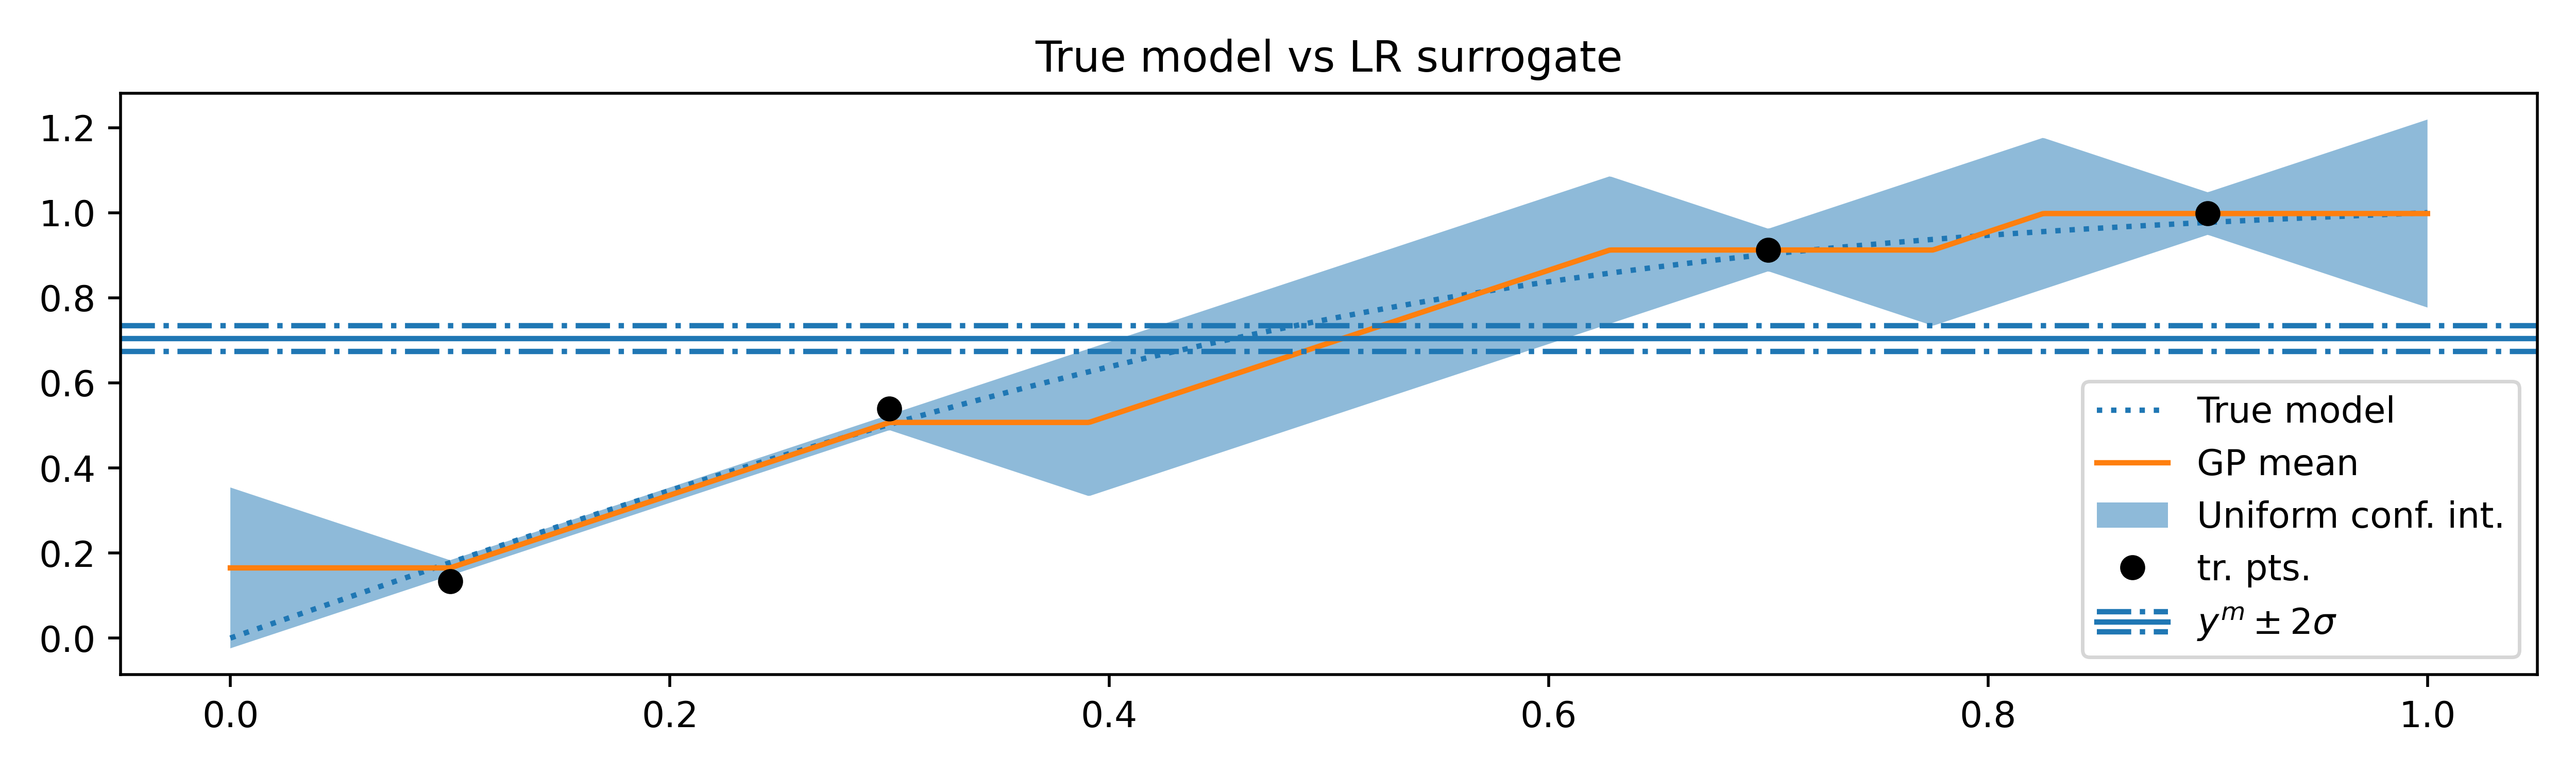
\includegraphics[width = 360pt]{results/pictures/d1/LR_model_comparison.png}
    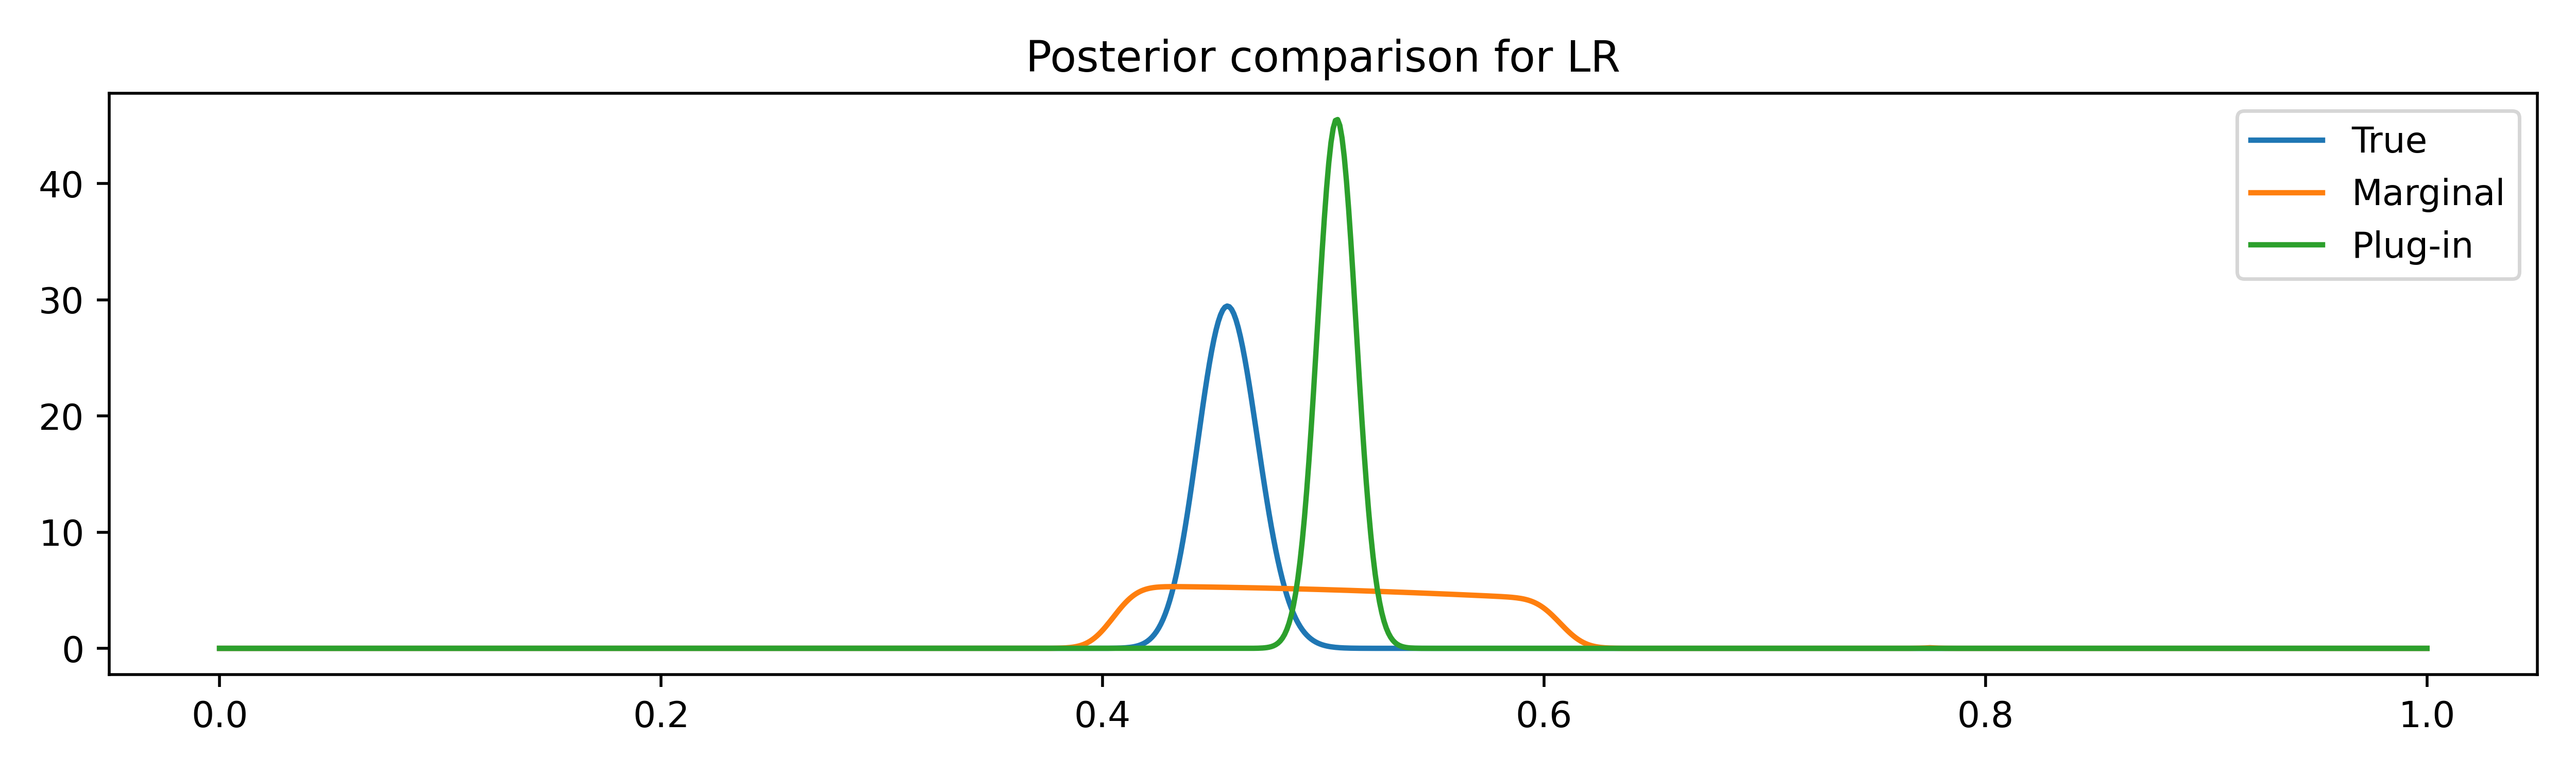
\includegraphics[width = 360pt]{results/pictures/d1/LR_posterior_comparison.png}
    \end{center}
    
    \caption{Impact of the plug-in likelihood~\eqref{eq:plug-in-likelihood} and LR-based marginal likelihood~\eqref{eq:LR-likelihood} on the posterior on the same IP as in Figure~\ref{fig:GP-likelihoods}. As for the GPR surrogate, the marginal likelihood~\eqref{eq:LR-likelihood} avoids an overconfident posteriors by preserving the surrogate's uncertainty.} 
    \label{fig:LR-likelihoods}
\end{figure}  

Picture~\ref{fig:LR-likelihoods} depicts the difference between the plug-in and the marginalized likelihoods for the simple one-dimensional case already presented in Section~\ref{sec:GPlike}. 
In the 1-d case, the LR mean is piecewise linear, resulting in a piecewise Gaussian plugin likelihood; the marginal likelihood is instead smoother.